%-*- coding=utf-8 -*-
\documentclass[UTF8]{ctexart}

\usepackage{geometry}
\usepackage{graphicx}
\usepackage{listings}
\usepackage{algorithm}
\usepackage{color}

\usepackage{algorithmic}
\usepackage[colorlinks,linkcolor=blue]{hyperref}

\definecolor{dkgreen}{rgb}{0,0.6,0}
\definecolor{gray}{rgb}{0.5,0.5,0.5}
\definecolor{mauve}{rgb}{0.58,0,0.82}
\lstset{ %
    aboveskip=3mm,
    belowskip=3mm,
    showstringspaces=false,
    columns=flexible,
    basicstyle={\small\ttfamily},
    numbers=left,
    numberstyle=\tiny\color{gray},
    keywordstyle=\color{blue},
    commentstyle=\color{dkgreen},
    stringstyle=\color{mauve},
    breaklines=true,
    breakatwhitespace=true,
    tabsize=3
}
\geometry{left=3.18cm,right=3.18cm,top=2.54cm,bottom=2.54cm}
\pagestyle{plain}   
% \usepackage{booktabs}
% \usepackage{subfigure}
\usepackage{setspace}
\date{}
\begin{document}

\begin{center}
    \quad \\
    \quad \\
    \huge  assignment1 report
\end{center}
\vskip 3.5cm

\begin{center}
    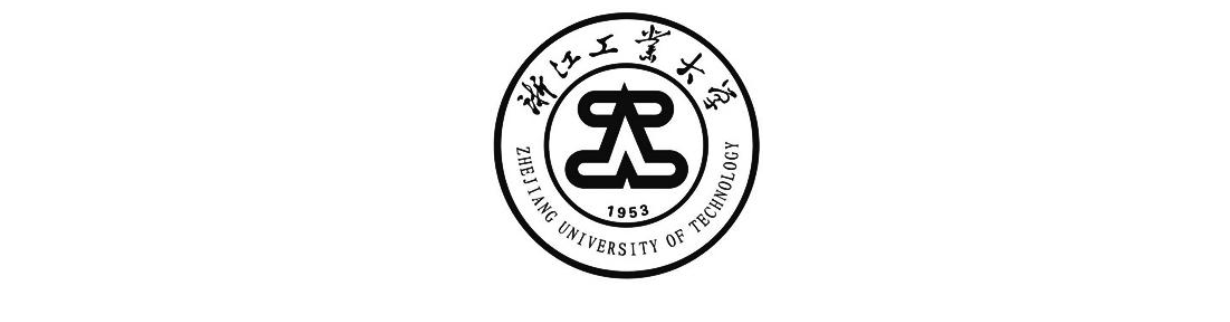
\includegraphics[scale=0.6]{../img/logo.png}
\end{center}
\vskip 4.5cm

\begin{quotation}
    \songti \fontsize{15}{15}
    \doublespacing
    \par\setlength\parindent{6.5em}
    \quad

    学\hspace{0.61cm} 院:\underline{\quad 计算机科学与技术学院、软件学院}

    专\hspace{0.61cm} 业:\underline{\qquad 软件工程(中外合作)\qquad\qquad  }

    学生姓名:\underline{\qquad\qquad\qquad 李肖 \qquad\qquad\qquad\qquad }

    学\hspace{0.61cm} 号:\underline{\qquad\qquad 202003340111 \qquad\qquad\qquad}

    \vskip 1cm
    \centering
    2022年11月26日
\end{quotation}

\newpage
\section{贪心算法}
\subsection{贪心算法的实现}
在这个题目中,我们先计算每个物品的单位重量价值,
然后按照单位重量价值从大到小排序,然后从大到小依次放入背包中,直到背包装满为止。具体代码如下:
\subsection{伪代码实现}
\begin{algorithm}
    \caption{Greedy algorithm}
    \label{alg3}
    \begin{algorithmic}[1]
        \REQUIRE $n$个物品,$m$个背包容量
        \ENSURE $m$个背包的最大价值
        \STATE \textbf{call} \textit{sort}($n$个物品, 根据物品单位重量价值从大到小排序)
        \FOR {$j \gets 1$; $j < n$; $j++$ }
        \FOR {$i \gets 1$; $i < m$; $i++$ }
        \IF {物品$i$没有被放入背包中 $\&\&$ 背包$j$剩余容量大于物品$i$的重量}
        \STATE 物品$i$放入背包$j$中
        \ENDIF
        \ENDFOR
        \ENDFOR

        \STATE \textbf{Output} $m$个背包的最大价值
    \end{algorithmic}
\end{algorithm}

\subsection{代码实现}
\lstinputlisting[language=C++]{../../code/greedy.cpp}

\section{领域搜索算法}
\subsection{领域搜索算法的实现}
在这个题目中,我们首先先规定一个初始解。在这个题目里面,我们将贪心算法的结果作为初始解

然后我们规定一个输入变量,这里我们定义一个数组 solution,solution[i]表示第i个物品放入哪个背包中,
solution[i] = -1表示第i个物品没有放入背包中,solution[i] = j表示第i个物品放入了第j个背包中。

然后根据这个输入变量,我们可以得到在背包中的物品的总价值。

我们将贪心算法得到的一个 solution 数组作为初始解,然后我们对 solution 数组进行变异,产生领域。
我这里使用了这么几种变异策略,对于所有没有塞入背包的物品 object

\begin{itemize}
    \item 如果一个物品有空位直接塞进去
    \item 如果一个背包中的一个物品被移除了以后,再把 object 塞入能得到更大的价值,就把这个物品移除后再塞入 object
    \item 如果一个背包 A 中的一个物品可以被转移到别的背包里,那么就转移这个物品到别的背包后,再塞入 object
    \item 如果一个背包 A 中的一个物品 1 可以在背包 B 中的一个物品2被移除后放入,那么就把物品 2 移除后塞入 物品1,再把 object 塞入背包1
\end{itemize}

然后我们对所有的领域进行评估,选择最优的领域作为下一步的输入变量,然后重复上述过程,直到有一次评估领域的时候得不到更优解结束。

\subsection{伪代码实现}
\begin{algorithm}
    \caption{neighborhood search algorithm}
    \label{alg3}
    \begin{algorithmic}[1]
        \REQUIRE $n$个物品,$m$个背包
        \ENSURE $m$个背包的最大价值
        \STATE \textbf{call} \textit{greedyAlgorithm}(n个物品, m个背包)
        \STATE $solution \gets $ \textit{getSolution}(m个背包)
        \WHILE {没有找到最优解}
        \STATE $neighborhood \gets $ \textit{getNeighborhood}(solution)
        \STATE $bestNeighbor \gets $ \textit{evaluate}(neighborhood)
        \IF {bestNeighbor的价值大于solution的价值}
        \STATE $solution \gets bestNeighbor$
        \ELSE
        \STATE \textbf{break}
        \ENDIF
        \ENDWHILE
    \end{algorithmic}
\end{algorithm}

\subsection{代码实现}
\lstinputlisting[language=C++]{../../code/improving_search.cpp}

\section{禁忌搜索}
\subsection{禁忌搜索的实现}
禁忌搜索的实现和领域搜索算法的实现类似,只是在领域搜索算法的基础上加入了禁忌表,禁忌表中存储了一些不应该被选择的解。
每次选择领域的时候,我们都会检查禁忌表,如果禁忌表中有这个解,那么就不选择这个解。

每次找到局部最优解的时候,就将全局最优解放入禁忌表里。

然后再用局部最优解和当前的全局最优解比较,如果局部最优解的价值更大,那么就更新全局最优解。

其中禁忌表有一禁忌长度,一旦禁忌表中的元素超出了这个禁忌长度,那么就从禁忌表中删除最开头的元素。

然后就是一旦禁忌表最开头的元素可以赋值给 solution 变量,起到一个回溯的作用,因为有的时候会走到一个无论怎么走都得不到全局最优解的地方
这个时候我们需要适当的回溯,因为这这个时候禁忌表中还存在这个 solution 附近的一个局部最优解,那么这次回溯以后不会找到这个 solution 附近的局部最优解,
反而能够往别的局部最优解方向跳转,提高搜索到全局最优解的可能行。

\newpage
\subsection{伪代码实现}

\begin{algorithm}
    \caption{tabu search algorithm}
    \begin{algorithmic}[1]
        \REQUIRE $n$个物品,$m$个背包
        \ENSURE $m$个背包的最大价值
        \STATE \textbf{call} \textit{greedyAlgorithm}(n个物品, m个背包)
        \STATE $solution \gets $ \textit{getSolution}(m个背包)
        \STATE $iteration \gets 1000$
        \STATE $tabuList \gets [\quad]$
        \STATE $neighborhood \gets [\quad]$
        \STATE $tabuLen \gets $n$ / 2$
        \WHILE {没有找到最优解}
        \WHILE {还能生成新的解}
        \STATE $neighbor \gets $ \textit{generateNeighbor}(solution)
        \IF {neighbor not in tabuList}
        \STATE $neighborhood \gets neighborhood + neighbor$
        \ENDIF
        \ENDWHILE

        \STATE $bestNeighbor \gets $ \textit{evaluate}(neighborhood)
        \IF {bestNeighbor的价值大于solution的价值}
        \STATE $solution \gets bestNeighbor$
        \STATE $tabuList \gets $ \textit{addTabuList}(tabuList, bestNeighbor, tabuLen)
        \IF {tabuList.size() > tabuLen}
        \STATE solution = tabuList[0]
        \STATE tabuList.popFront()
        \ENDIF
        \ENDIF
        \ENDWHILE
    \end{algorithmic}
\end{algorithm}

\lstinputlisting[language=C++]{../../code/tabu.cpp}

\newpage
\section{算法正确性证明}

\subsection{输入数据1}
\lstinputlisting[numbers=none]{../../code/data/data2}

\noindent
\textbf{greedy algorithm 结果}

\begin{lstlisting}[numbers=none]
Knapsack 0 used 10 of 11
Knapsack 1 used 7 of 7
Knapsack 2 used 3 of 6
Knapsack 3 used 0 of 6
Knapsack 4 used 0 of 6
Result: 121
\end{lstlisting}

\noindent
\textbf{neighborhood search algorithm 结果}

\begin{lstlisting}[numbers=none]
Knapsack 0 used 11 of 11
Knapsack 1 used 7 of 7
Knapsack 2 used 3 of 6
Knapsack 3 used 6 of 6
Knapsack 4 used 0 of 6
Result: 129
\end{lstlisting}

\noindent
\textbf{tabu search algorithm 结果}

\begin{lstlisting}[numbers=none]
Knapsack 0 used 9 of 11
Knapsack 1 used 7 of 7
Knapsack 2 used 3 of 6
Knapsack 3 used 6 of 6
Knapsack 4 used 3 of 6
Result: 148
\end{lstlisting}

\newpage
\subsection{输入数据2}
\lstinputlisting[numbers=none]{../../code/data/data3}

\noindent
\textbf{greedy algorithm 结果}

\begin{lstlisting}[numbers=none]
Knapsack 0 used 10 of 12
Knapsack 1 used 10 of 11
Knapsack 2 used 4 of 8
Knapsack 3 used 0 of 7
Result: 53
\end{lstlisting}

\noindent
\textbf{neighborhood search algorithm 结果}

\begin{lstlisting}[numbers=none]
Knapsack 0 used 10 of 12
Knapsack 1 used 11 of 11
Knapsack 2 used 4 of 8
Knapsack 3 used 7 of 7
Result: 55
\end{lstlisting}

\noindent
\textbf{tabu search algorithm 结果}

\begin{lstlisting}[numbers=none]
Knapsack 0 used 9 of 12
Knapsack 1 used 11 of 11
Knapsack 2 used 4 of 8
Knapsack 3 used 7 of 7
Result: 64
\end{lstlisting}

\newpage
\subsection{输入数据3}
\lstinputlisting[numbers=none]{../../code/data/data4}

\noindent
\textbf{greedy algorithm 结果}

\begin{lstlisting}[numbers=none]
Knapsack 0 used 1 of 2
Knapsack 1 used 5 of 6
Knapsack 2 used 4 of 8
Knapsack 3 used 14 of 17
Knapsack 4 used 6 of 7
Result: 166
\end{lstlisting}

\noindent
\textbf{neighborhood search algorithm 结果}

\begin{lstlisting}[numbers=none]
Knapsack 0 used 1 of 2
Knapsack 1 used 5 of 6
Knapsack 2 used 8 of 8
Knapsack 3 used 14 of 17
Knapsack 4 used 4 of 7
Result: 170
\end{lstlisting}

\noindent
\textbf{tabu search algorithm 结果}
\begin{lstlisting}[numbers=none]
Knapsack 0 used 0 of 2
Knapsack 1 used 6 of 6
Knapsack 2 used 8 of 8
Knapsack 3 used 17 of 17
Knapsack 4 used 7 of 7
Result: 176
\end{lstlisting}

\end{document}